% KemdiCode MCP Server — IEEE Journal Paper v1.25.0
% Copyright (C) 2025-2026 Kemdi Sp. z o.o. (Dawid Irzyk)
% Licensed under GNU GPL v3

\documentclass[journal,10pt]{IEEEtran}

% ── Packages ──────────────────────────────────────────────────────
\usepackage[utf8]{inputenc}
\usepackage[T1]{fontenc}
\usepackage[english]{babel}
\usepackage{amsmath,amssymb}
\usepackage{graphicx}
\usepackage{tikz}
\usetikzlibrary{arrows.meta,positioning,fit,calc,shapes.geometric,decorations.pathreplacing,backgrounds,patterns}
\usepackage{booktabs}
\usepackage{tabularx}
\usepackage{multirow}
\usepackage{enumitem}
\usepackage{listings}
\usepackage{microtype}
\usepackage{cite}
\usepackage[ruled,linesnumbered,noend]{algorithm2e}
\usepackage{url}
\usepackage{hyperref}
\hypersetup{
  colorlinks=false,
  pdfborder={0 0 0},
  pdftitle={KemdiCode MCP: A Multi-Layer Protocol Server for AI-Assisted Software Engineering},
  pdfauthor={Dawid Irzyk},
}

% ── B&W color definitions ────────────────────────────────────────
\definecolor{darkgray}{gray}{0.25}
\definecolor{medgray}{gray}{0.55}
\definecolor{lightgray}{gray}{0.85}
\definecolor{verylightgray}{gray}{0.93}
\definecolor{codebg}{gray}{0.95}

% ── Listings ─────────────────────────────────────────────────────
\lstset{
  basicstyle=\ttfamily\scriptsize,
  backgroundcolor=\color{codebg},
  frame=single,
  rulecolor=\color{medgray},
  breaklines=true,
  tabsize=2,
  columns=fullflexible,
  xleftmargin=2mm,
  framexleftmargin=2mm,
  aboveskip=6pt,
  belowskip=4pt,
}

% ── Helpers ──────────────────────────────────────────────────────
\newcommand{\doi}[1]{\href{https://doi.org/#1}{\texttt{doi:#1}}}
\newcommand{\code}[1]{\texttt{#1}}
\newcommand{\layerthree}{L\textsubscript{3}}
\newcommand{\layertwo}{L\textsubscript{2}}
\newcommand{\layerone}{L\textsubscript{1}}

% ══════════════════════════════════════════════════════════════════
\begin{document}

\title{KemdiCode MCP: A Multi-Layer Protocol Server\\for AI-Assisted Software Engineering}

\author{Dawid~Irzyk%
\thanks{D. Irzyk is with Kemdi Sp. z o.o., Poland (e-mail: dawid@kemdi.pl).}%
\thanks{This work is licensed under the GNU General Public License v3.0. Source code is available at \url{https://git.kemdi.pl}.}}

\markboth{Kemdi Technical Report, 2026}%
{Irzyk: KemdiCode MCP: A Multi-Layer Protocol Server for AI-Assisted Software Engineering}

\maketitle

% ── Abstract ─────────────────────────────────────────────────────
\begin{abstract}
This paper presents KemdiCode MCP Server, an open-source implementation of the Model Context Protocol~(MCP) that extends the specification with 142~specialized tools, a three-layer distributed bus architecture, a persistent cognition subsystem, and multi-provider LLM orchestration across eight providers. The server communicates with IDE clients via JSON-RPC~2.0 over HTTP with Server-Sent Events. We describe in detail the protocol stack comprising three communication layers --- \layerthree~ClusterBus for inter-cluster Redis Pub/Sub signaling with HMAC authentication and bloom-filter deduplication, \layertwo~DataFlowBus for typed inter-module messaging with Zod-validated envelopes, and \layerone~GlobalEventBus for in-process event propagation with chain-depth limiting. We formalize the anti-amplification bridge mechanism, the LLM Magistrale's multi-strategy aggregation with a composite scoring function, and the self-regulating PassController. The cognition subsystem provides cross-session AI self-awareness through eight interconnected stores with reactive event handlers. Experimental validation confirms 559~passing tests and compatibility with four major MCP clients. Version~1.25.0 introduces cluster-bus hardening with circuit breakers, bloom-filter deduplication, and signal-flow backpressure control.
\end{abstract}

\begin{IEEEkeywords}
Model Context Protocol, large language models, multi-agent systems, distributed systems, software engineering tools, AI-assisted development
\end{IEEEkeywords}

% ══════════════════════════════════════════════════════════════════
\section{Introduction}
\label{sec:intro}

\IEEEPARstart{M}{odern} AI-assisted development tools require deep integration between Large Language Models~(LLMs) and the developer's working environment. The Model Context Protocol~(MCP)~\cite{mcp2024}, introduced by Anthropic in November~2024 and formalized in specification version~2025-11-25~\cite{mcpspec2025}, standardizes the interface between AI clients and tool servers using JSON-RPC~2.0~\cite{jsonrpc2} as the transport protocol. However, reference implementations typically provide a narrow set of tools with limited state management and no inter-session persistence.

KemdiCode MCP Server addresses these limitations by extending the MCP paradigm along five dimensions:

\begin{enumerate}[nosep,label=(\roman*)]
  \item \emph{Comprehensive tooling}: 142~tools across 23~categories covering the full software engineering lifecycle, from code analysis and AST-based editing to distributed task management.
  \item \emph{Persistent cognition}: AI agents retain decision history, confidence calibration, error patterns, and mental models across sessions through Redis-backed stores with configurable TTLs.
  \item \emph{Distributed execution}: A three-layer bus architecture enables multi-cluster LLM orchestration with quality-driven aggregation and anti-amplification safeguards.
  \item \emph{Multi-agent coordination}: Redis-backed kanban boards, workspaces, agent registration, and Pub/Sub message passing support collaborative multi-session workflows.
  \item \emph{Provider-agnostic LLM routing}: Eight providers with native and OpenAI-compatible adapters, fallback chains, cost optimization, and Zod-schema structured output.
\end{enumerate}

The remainder of this paper is organized as follows. Section~\ref{sec:related} surveys related work. Section~\ref{sec:arch} presents the system architecture. Section~\ref{sec:protocol} provides a detailed technical description of all three protocol layers with formal specifications. Section~\ref{sec:magistrale} describes the LLM Magistrale. Section~\ref{sec:cognition} covers the cognition subsystem. Section~\ref{sec:tools} catalogs the tool categories. Section~\ref{sec:multiagent} describes multi-agent coordination. Section~\ref{sec:security} addresses security mechanisms. Section~\ref{sec:eval} presents the evaluation. Section~\ref{sec:conclusion} concludes.

% ══════════════════════════════════════════════════════════════════
\section{Related Work}
\label{sec:related}

The Model Context Protocol builds on the architectural patterns established by the Language Server Protocol~(LSP)~\cite{lsp2016}, which standardized language intelligence features across IDEs. While LSP focuses on language-specific operations (completion, diagnostics, refactoring), MCP generalizes the client-server pattern to arbitrary tool invocations for AI assistants.

Multi-agent LLM frameworks have been explored extensively in recent literature. AutoGen~\cite{wu2023autogen} enables multi-agent conversation through a conversable agent abstraction with customizable conversation patterns. MetaGPT~\cite{hong2023metagpt} introduces role-based agent coordination with structured output protocols. Li~et~al.~\cite{li2024multiagent} survey workflow patterns, infrastructure requirements, and open challenges in LLM-based multi-agent systems. Guo~et~al.~\cite{guo2024ijcai} provide a comprehensive taxonomy of multi-agent architectures, covering communication, memory, and planning mechanisms. KemdiCode differs from these frameworks by operating at the protocol level---it exposes coordination primitives as MCP tools rather than implementing a fixed agent architecture.

For distributed messaging, Redis Pub/Sub~\cite{redis} provides the foundation for KemdiCode's inter-cluster communication, following patterns described by Lamport~\cite{lamport1978} for event ordering in distributed systems. The bloom filter~\cite{bloom1970} is employed for probabilistic deduplication in the cluster bus. Tree-sitter~\cite{treesitter}, based on the incremental parsing techniques of Wagner and Graham~\cite{wagner1998}, provides the AST infrastructure. Secret sharing follows Shamir's original construction~\cite{shamir1979}.

% ══════════════════════════════════════════════════════════════════
\section{System Architecture}
\label{sec:arch}

Fig.~\ref{fig:arch} shows the high-level system architecture. The server is organized into six layers: transport, session management, tool registry, bus architecture, shared infrastructure, and cognition.

\begin{figure}[!t]
\centering
\resizebox{\columnwidth}{!}{%
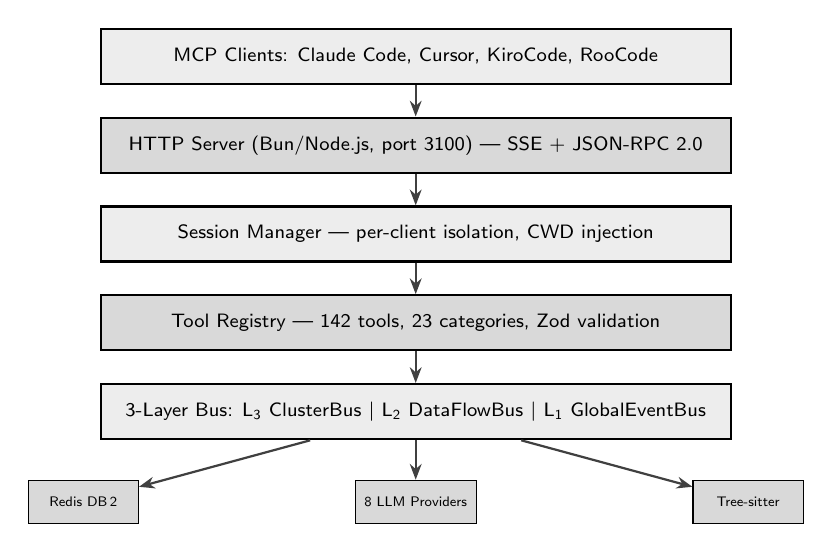
\begin{tikzpicture}[
  node distance=0.4cm,
  box/.style={draw, thick, minimum width=80mm, minimum height=7mm, font=\sffamily\scriptsize, align=center, fill=#1},
  smallbox/.style={draw, minimum width=14mm, minimum height=5.5mm, font=\sffamily\tiny, align=center, fill=#1},
  arr/.style={-{Stealth[length=2mm]}, thick, color=darkgray},
]
  \node[box=verylightgray] (clients) {MCP Clients: Claude Code, Cursor, KiroCode, RooCode};
  \node[box=lightgray, below=of clients] (http) {HTTP Server (Bun/Node.js, port 3100) --- SSE + JSON-RPC 2.0};
  \node[box=verylightgray, below=of http] (session) {Session Manager --- per-client isolation, CWD injection};
  \node[box=lightgray, below=of session] (registry) {Tool Registry --- 142 tools, 23 categories, Zod validation};
  \node[box=verylightgray, below=of registry] (bus) {3-Layer Bus: \layerthree{} ClusterBus $\mid$ \layertwo{} DataFlowBus $\mid$ \layerone{} GlobalEventBus};
  \node[smallbox=lightgray, below left=0.5cm and -0.5cm of bus] (redis) {Redis DB\,2};
  \node[smallbox=lightgray, below=0.5cm of bus] (llm) {8 LLM Providers};
  \node[smallbox=lightgray, below right=0.5cm and -0.5cm of bus] (ts) {Tree-sitter};

  \draw[arr] (clients) -- (http);
  \draw[arr] (http) -- (session);
  \draw[arr] (session) -- (registry);
  \draw[arr] (registry) -- (bus);
  \draw[arr] (bus) -- (redis);
  \draw[arr] (bus) -- (llm);
  \draw[arr] (bus) -- (ts);
\end{tikzpicture}}%
\caption{High-level system architecture showing the six-layer stack from client to infrastructure.}
\label{fig:arch}
\end{figure}

\subsection{Transport Layer}

The server implements the MCP Streamable~HTTP transport, exposing the endpoints listed in Table~\ref{tab:endpoints}. Communication follows JSON-RPC~2.0 with the MCP method extensions (\code{tools/list}, \code{tools/call}, \code{initialize}, \code{notifications/initialized}, etc.). Server-Sent Events~(SSE) provide the server-to-client notification channel with configurable keep-alive intervals.

\begin{table}[!t]
\centering
\caption{HTTP Endpoints}
\label{tab:endpoints}
\begin{tabular}{@{}llp{32mm}@{}}
\toprule
\textbf{Method} & \textbf{Path} & \textbf{Purpose} \\
\midrule
\texttt{GET}  & \texttt{/sse}        & SSE notification stream \\
\texttt{POST} & \texttt{/message}    & JSON-RPC tool invocations \\
\texttt{GET}  & \texttt{/stream/:id} & Per-request execution stream \\
\texttt{GET}  & \texttt{/health}     & Health check and uptime \\
\texttt{GET}  & \texttt{/tools}      & Tool listing with schemas \\
\texttt{GET}  & \texttt{/mcp}        & Streamable HTTP endpoint \\
\bottomrule
\end{tabular}
\end{table}

\subsection{Tool Registry}

The tool registry manages 142~tools through a unified \code{UnifiedTool} interface. Each tool defines its input schema using Zod~\cite{zod}, which is converted to JSON~Schema for the MCP protocol. A non-trivial conversion handles Zod's \code{discriminatedUnion} type: since many MCP clients cannot process JSON~Schema \code{oneOf} constructs, the registry flattens discriminated union variants into a single merged object schema via \code{toMcpInputSchema()}.

Tool annotations follow the MCP specification's hint system with three boolean flags: \code{readOnlyHint} (tool does not modify state), \code{destructiveHint} (tool may delete data), and \code{openWorldHint} (tool accesses external services). These annotations are maintained in a centralized map (\code{annotations-map.ts}) and attached during schema generation.

Lazy loading ensures that tool implementations are instantiated on first invocation. A background warmup phase pre-loads all schemas after server start and emits \code{tools/list\_changed} notifications to connected clients. The availability checker reports tool health with soft and force modes, suggesting fallback alternatives when a tool's dependencies are unavailable.

% ══════════════════════════════════════════════════════════════════
\section{Protocol Layer Architecture}
\label{sec:protocol}

The communication infrastructure consists of three layers connected by anti-amplification bridges. Each layer operates at a distinct scope and employs different transport mechanisms. Fig.~\ref{fig:bus} illustrates the layered design with bridge interconnections.

\begin{figure}[!t]
\centering
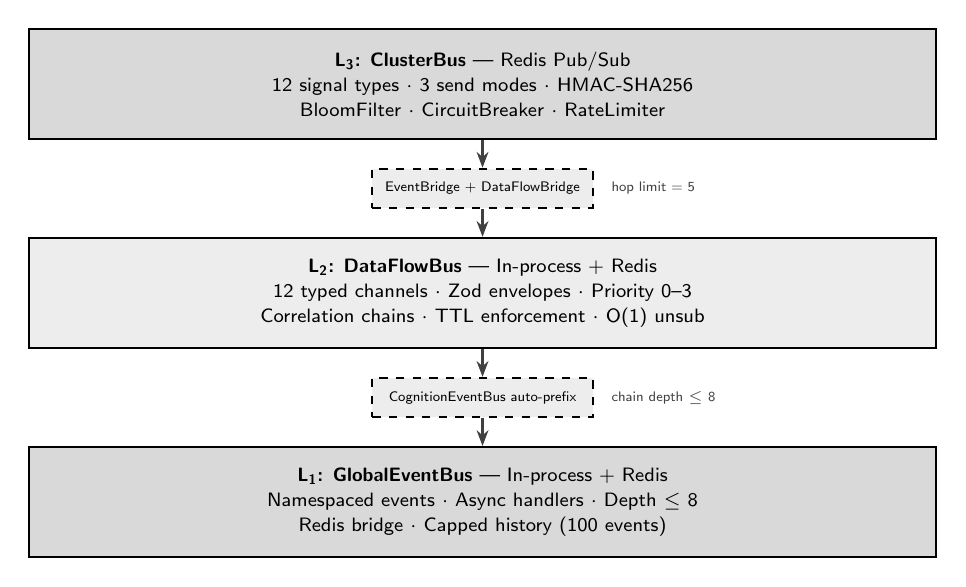
\begin{tikzpicture}[
  node distance=0.35cm,
  layer/.style={draw, thick, minimum width=\columnwidth-6mm, font=\sffamily\scriptsize, align=center, minimum height=14mm},
  bridge/.style={draw, dashed, thick, minimum width=28mm, minimum height=5mm, font=\sffamily\tiny, fill=verylightgray},
  arr/.style={-{Stealth[length=2mm]}, thick, color=darkgray},
]
  % L3
  \node[layer, fill=lightgray] (l3) {
    \textbf{\layerthree: ClusterBus} --- Redis Pub/Sub\\[1pt]
    12 signal types $\cdot$ 3 send modes $\cdot$ HMAC-SHA256\\[1pt]
    BloomFilter $\cdot$ CircuitBreaker $\cdot$ RateLimiter
  };

  \node[bridge, below=of l3] (b32) {EventBridge + DataFlowBridge};

  \node[layer, fill=verylightgray, below=of b32] (l2) {
    \textbf{\layertwo: DataFlowBus} --- In-process + Redis\\[1pt]
    12 typed channels $\cdot$ Zod envelopes $\cdot$ Priority 0--3\\[1pt]
    Correlation chains $\cdot$ TTL enforcement $\cdot$ O(1) unsub
  };

  \node[bridge, below=of l2] (b21) {CognitionEventBus auto-prefix};

  \node[layer, fill=lightgray, below=of b21] (l1) {
    \textbf{\layerone: GlobalEventBus} --- In-process + Redis\\[1pt]
    Namespaced events $\cdot$ Async handlers $\cdot$ Depth $\leq$ 8\\[1pt]
    Redis bridge $\cdot$ Capped history (100 events)
  };

  \draw[arr] (l3.south) -- (b32.north);
  \draw[arr] (b32.south) -- (l2.north);
  \draw[arr] (l2.south) -- (b21.north);
  \draw[arr] (b21.south) -- (l1.north);

  \node[font=\sffamily\tiny, right=1mm of b32, text=darkgray] {hop limit = 5};
  \node[font=\sffamily\tiny, right=1mm of b21, text=darkgray] {chain depth $\leq$ 8};
\end{tikzpicture}
\caption{Three-layer bus architecture with anti-amplification bridges. Arrows indicate the primary message flow direction; bidirectional bridging is supported with hop-count guards.}
\label{fig:bus}
\end{figure}

\subsection{\layerthree: ClusterBus --- Inter-Cluster Communication}
\label{sec:l3}

The ClusterBus enables inter-cluster communication over Redis Pub/Sub~\cite{redis}. It is the only layer that crosses process boundaries, making it the primary mechanism for distributed LLM orchestration and multi-node coordination.

\subsubsection{Signal Structure}

Every message on the ClusterBus is a \code{ClusterSignal} with the following structure:

\begin{lstlisting}[language={}]
ClusterSignal {
  id:        string    // UUID v4
  type:      SignalType // 12 enum values
  source:    string    // originating node ID
  target?:   string    // unicast target
  payload:   unknown   // type-dependent data
  timestamp: number    // Unix ms
  ttl:       number    // max hops
  priority:  0|1|2|3   // 0=lowest, 3=critical
  metadata:  Record<string, unknown>
  hmac?:     string    // HMAC-SHA256 signature
}
\end{lstlisting}

The 12~signal types are organized into four namespaces, shown in Table~\ref{tab:signals}.

\begin{table}[!t]
\centering
\caption{ClusterBus Signal Types}
\label{tab:signals}
\begin{tabular}{@{}lp{45mm}@{}}
\toprule
\textbf{Namespace} & \textbf{Types} \\
\midrule
\code{llm:*}     & \code{request}, \code{result}, \code{stream-chunk}, \code{error} \\
\code{cluster:*} & \code{join}, \code{leave}, \code{heartbeat} \\
\code{data:*}    & \code{broadcast}, \code{unicast} \\
\code{control:*} & \code{pause}, \code{resume}, \code{config} \\
\bottomrule
\end{tabular}
\end{table}

\subsubsection{Send Modes}

Three send modes are supported:

\begin{description}[nosep,style=unboxed,leftmargin=0pt,font=\normalfont\itshape]
\item[Unicast.] The signal carries a \code{target} field specifying the destination node ID. Only the targeted node processes the signal; others discard it after deduplication.
\item[Broadcast.] The \code{target} field is omitted. All subscribed nodes receive and process the signal.
\item[Routed.] The signal is dispatched via the MetaRouter, which evaluates tag-based routing rules with AND/OR boolean logic. Route patterns support regex matching (capped at 200~characters to prevent ReDoS).
\end{description}

\subsubsection{Dual-Layer Deduplication}

The ClusterBus employs a dual-layer deduplication strategy to prevent duplicate signal processing:

\begin{enumerate}[nosep]
\item \emph{Recent set}: A bounded set of the most recent 2{,}000 signal IDs provides exact deduplication for recently received signals with O(1) lookup.
\item \emph{Bloom filter}: A space-efficient probabilistic filter~\cite{bloom1970} configured for 20{,}000~items at a false-positive rate of 0.1\%, occupying approximately 35\,KB of memory. The filter uses the formula:
\end{enumerate}

\begin{equation}
m = -\frac{n \ln p}{(\ln 2)^2}, \quad k = \frac{m}{n} \ln 2
\label{eq:bloom}
\end{equation}

\noindent where $n$ is the expected item count, $p$ is the target false-positive rate, $m$ is the bit array size, and $k$ is the number of hash functions. At the configured parameters ($n=20{,}000$, $p=0.001$), this yields $m \approx 287{,}552$ bits and $k \approx 10$ hash functions.

When the recent set reaches capacity, its oldest entries are migrated to the bloom filter before eviction. This two-tier approach achieves zero false positives for recent signals while providing memory-bounded probabilistic deduplication for the long tail.

\subsubsection{HMAC Authentication}

Signals are authenticated using HMAC-SHA256. The signing process computes:

\begin{equation}
\text{HMAC} = H_K\bigl(\text{id} \| \text{type} \| \text{source} \| \text{timestamp}\bigr)
\label{eq:hmac}
\end{equation}

\noindent where $H_K$ denotes HMAC-SHA256 with shared key $K$, and $\|$ denotes string concatenation. Verification uses constant-time comparison via the runtime's \code{timingSafeEqual()} function to prevent timing side-channel attacks. Signals failing HMAC verification are silently dropped and logged.

\subsubsection{SignalFlowController}

The SignalFlowController governs the throughput and reliability of signal processing through four mechanisms:

\begin{description}[nosep,style=unboxed,leftmargin=0pt,font=\normalfont\itshape]
\item[Rate Limiting.] A sliding-window rate limiter with 1-second windows caps the number of signals processed per window. Excess signals are either buffered or dropped based on the configured backpressure policy.

\item[Circuit Breaker.] Implements the standard three-state pattern (closed, open, half-open) with configurable thresholds:
\begin{itemize}[nosep]
  \item Failure threshold: 10~consecutive failures to transition from closed to open.
  \item Open duration: 5{,}000\,ms before transitioning to half-open.
  \item Half-open probes: 2~successful signals required to return to closed.
\end{itemize}

\item[Priority Filtering.] Signals carry a priority field (0--3). Under backpressure, the controller drops low-priority signals first, ensuring critical signals (priority~3) are always processed.

\item[Backpressure.] Queue depth is monitored continuously. When the queue exceeds the high-water mark, the controller transitions to a backpressure state, activating priority filtering and signaling upstream nodes to reduce their send rate.
\end{description}

\subsubsection{MetaRouter}

The MetaRouter provides tag-based signal routing with boolean logic. Routing rules specify:

\begin{lstlisting}[language={}]
RouteRule {
  pattern:  string   // regex (max 200 chars)
  tags:     string[] // required meta tags
  logic:    "AND" | "OR"
  target:   string   // destination node/group
  priority: number
}
\end{lstlisting}

Rules are evaluated in priority order. The first matching rule determines the signal's destination. Regex patterns are length-capped to prevent ReDoS attacks.

\subsubsection{HealthMonitor}

Each node emits periodic heartbeat signals (type \code{cluster:heartbeat}). The HealthMonitor tracks:

\begin{itemize}[nosep]
\item Last heartbeat timestamp per node.
\item Latency statistics (moving average).
\item Stale detection: nodes exceeding the heartbeat timeout (default 30\,s) are marked stale and excluded from routing decisions.
\item Automatic pruning of stale entries with O(1) unsubscribe via \code{Map}-based tracking.
\end{itemize}

\subsection{\layertwo: DataFlowBus --- Inter-Module Communication}
\label{sec:l2}

The DataFlowBus provides typed, schema-validated messaging between server modules. It operates primarily in-process but persists messages to Redis for cross-session access.

\subsubsection{Channel Architecture}

The bus defines 12~typed channels organized into four domains, as shown in Table~\ref{tab:channels}.

\begin{table}[!t]
\centering
\caption{DataFlowBus Channels}
\label{tab:channels}
\begin{tabular}{@{}lp{42mm}@{}}
\toprule
\textbf{Domain} & \textbf{Channels} \\
\midrule
AI        & \code{ai:completion}, \code{ai:structured}, \code{ai:research} \\
Kanban    & \code{kanban:task-change}, \code{kanban:complexity} \\
Cognition & \code{cognition:decision}, \code{cognition:intent}, \code{cognition:error} \\
Agent     & \code{agent:status}, \code{agent:message} \\
System    & \code{system:health}, \code{system:config} \\
\bottomrule
\end{tabular}
\end{table}

\subsubsection{Envelope Structure}

Every message is wrapped in a \code{DataFlowEnvelope}:

\begin{lstlisting}[language={}]
DataFlowEnvelope<T> {
  id:           string  // UUID v4
  channel:      Channel // one of 12 channels
  payload:      T       // Zod-validated data
  correlationId: string // request chain ID
  schemaVersion: string // semver
  priority:     0|1|2|3
  ttl:          number  // milliseconds
  source:       string  // originating module
  target?:      string  // optional filter
  sessionId?:   string
  agentId?:     string
  timestamp:    number
}
\end{lstlisting}

Payloads are validated against per-channel Zod schemas at publish time. Invalid payloads cause synchronous rejection with descriptive error messages.

\subsubsection{Subscription Management}

Subscribers register for specific channels and receive messages asynchronously. The implementation uses a \code{Map<string, Set<Callback>>} structure providing:

\begin{itemize}[nosep]
\item O(1) subscribe and unsubscribe operations.
\item Automatic cleanup of idle subscriptions after 60~minutes of inactivity.
\item Correlation-based filtering: subscribers may filter messages by \code{correlationId} to receive only messages belonging to a specific request chain.
\end{itemize}

\subsubsection{Redis Persistence}

Messages are persisted to Redis under the key pattern \code{mcp:dataflow:\{channel\}} as JSON-serialized envelopes. This enables cross-session message access and supports the multi-agent shared-context mechanism described in Section~\ref{sec:multiagent}.

\subsection{\layerone: GlobalEventBus --- In-Process Events}
\label{sec:l1}

The GlobalEventBus is a singleton, in-process event emitter with namespaced events following the pattern \code{module:category:action} (e.g., \code{cognition:decision:recorded}, \code{kanban:task:completed}).

\subsubsection{Event Dispatch}

Handlers execute asynchronously via \code{queueMicrotask()} with configurable priority. The dispatch algorithm:

\begin{enumerate}[nosep]
\item Increment chain depth counter.
\item Check $\text{depth} \leq \text{MAX\_EVENT\_CHAIN\_DEPTH}$ (configured as~8). If exceeded, log warning and discard.
\item Sort handlers by priority (descending).
\item Invoke each handler with \code{queueMicrotask()}, passing the event payload.
\item Decrement chain depth counter on completion.
\end{enumerate}

The chain depth limit of~8 prevents cascading event storms where handler~$A$ emits event~$e_1$, triggering handler~$B$ which emits~$e_2$, and so forth.

\subsubsection{Redis Bridge}

The Redis bridge propagates selected events across sessions:

\begin{itemize}[nosep]
\item Events matching configurable patterns are serialized and published to Redis Pub/Sub channels under \code{mcp:events:\{type\}}.
\item Incoming events from other sessions are deserialized and re-emitted on the local bus with a \code{\_remote} flag to prevent re-publication.
\item Failed publications are retried twice with exponential backoff (100\,ms, 200\,ms).
\item Event history is capped at 100~entries per type with a 1-hour TTL in Redis.
\end{itemize}

\subsection{Anti-Amplification Bridge Mechanism}
\label{sec:bridges}

Bridges connect the three layers, enabling signals originating at one scope to propagate to another. Without safeguards, bridges would create feedback loops: a signal bridged from \layerthree{} to \layerone{} could trigger an event that bridges back to \layerthree{}, creating infinite recursion.

Four anti-amplification mechanisms prevent this:

\begin{table}[!t]
\centering
\caption{Anti-Amplification Guards}
\label{tab:guards}
\begin{tabular}{@{}lp{40mm}@{}}
\toprule
\textbf{Guard} & \textbf{Mechanism} \\
\midrule
Hop counter    & Signals carry \code{\_bridgeHops}, incremented per crossing. Max = 5. \\
Source prefix  & Skip signals whose \code{source} starts with the bridge's own layer prefix. \\
Dedup set      & Per-bridge message-ID set prevents re-bridging. \\
Chain depth    & \layerone{} enforces depth $\leq$ 8, limiting cascades. \\
\bottomrule
\end{tabular}
\end{table}

The bridge mapping is summarized in Table~\ref{tab:bridgemap}.

\begin{table}[!t]
\centering
\caption{Bridge Signal Mappings}
\label{tab:bridgemap}
\begin{tabular}{@{}lll@{}}
\toprule
\textbf{Direction} & \textbf{Source Signal} & \textbf{Target} \\
\midrule
\layerthree$\to$\layertwo & \code{llm:result}  & \code{ai:completion} \\
\layerthree$\to$\layertwo & \code{data:*}      & \code{agent:message} \\
\layertwo$\to$\layerthree & \code{ai:research} & \code{llm:request} \\
\layerthree$\to$\layerone & \code{cluster:join} & \code{system:node-joined} \\
\layerone$\to$\layerthree & \code{system:alert} & \code{control:config} \\
\bottomrule
\end{tabular}
\end{table}

% ══════════════════════════════════════════════════════════════════
\section{LLM Magistrale}
\label{sec:magistrale}

The LLM Magistrale orchestrates distributed prompt execution across multiple clusters, each potentially backed by a different LLM provider. Fig.~\ref{fig:magistrale} illustrates the dispatch flow.

\begin{figure}[!t]
\centering
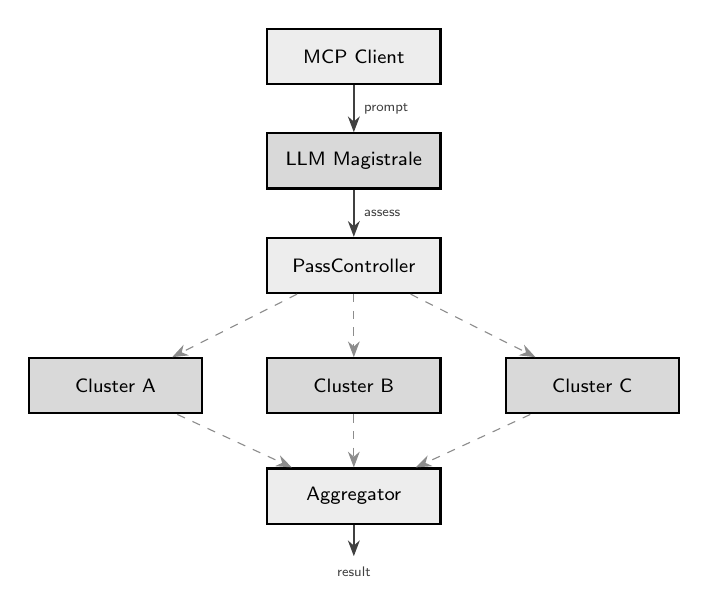
\begin{tikzpicture}[
  node distance=0.6cm,
  box/.style={draw, thick, minimum width=22mm, minimum height=7mm, font=\sffamily\scriptsize, align=center, fill=#1},
  arr/.style={-{Stealth[length=2mm]}, thick, color=darkgray},
  darr/.style={-{Stealth[length=2mm]}, dashed, color=medgray},
]
  \node[box=verylightgray] (client) {MCP Client};
  \node[box=lightgray, below=of client] (mag) {LLM Magistrale};
  \node[box=verylightgray, below=of mag] (pass) {PassController};

  \node[box=lightgray, below left=0.8cm and 0.8cm of pass] (ca) {Cluster A};
  \node[box=lightgray, below=0.8cm of pass] (cb) {Cluster B};
  \node[box=lightgray, below right=0.8cm and 0.8cm of pass] (cc) {Cluster C};

  \node[box=verylightgray, below=2.2cm of pass] (agg) {Aggregator};

  \draw[arr] (client) -- node[right, font=\sffamily\tiny] {prompt} (mag);
  \draw[arr] (mag) -- node[right, font=\sffamily\tiny] {assess} (pass);
  \draw[darr] (pass) -- (ca);
  \draw[darr] (pass) -- (cb);
  \draw[darr] (pass) -- (cc);
  \draw[darr] (ca) -- (agg);
  \draw[darr] (cb) -- (agg);
  \draw[darr] (cc) -- (agg);
  \draw[arr] (agg.south) -- ++(0,-0.4) node[below, font=\sffamily\tiny] {result};
\end{tikzpicture}
\caption{LLM Magistrale dispatch flow. Solid arrows indicate control flow; dashed arrows indicate asynchronous signal-based communication via the ClusterBus.}
\label{fig:magistrale}
\end{figure}

\subsection{Aggregation Strategies}

The Magistrale supports four aggregation strategies, selectable per request:

\begin{description}[nosep,style=unboxed,leftmargin=0pt,font=\normalfont\itshape]
\item[First-wins.] Returns the first response received, canceling remaining cluster requests. Optimizes for latency.

\item[Best-of-$n$.] Collects all $n$ responses and scores each using the composite scoring function (Section~\ref{sec:scoring}). Returns the highest-scoring response.

\item[Consensus.] Computes pairwise weighted Jaccard similarity between all responses. Requires agreement above a configurable threshold (default 0.6). If no consensus is reached, falls back to best-of-$n$.

\item[Fallback-chain.] Tries clusters sequentially in priority order. Returns the first successful response; continues to the next cluster on failure.
\end{description}

\subsection{Composite Scoring Function}
\label{sec:scoring}

The best-of-$n$ and consensus strategies evaluate responses using a weighted composite score:

\begin{equation}
S = w_q \cdot Q + w_d \cdot D + w_t \cdot T - w_l \cdot L
\label{eq:score}
\end{equation}

\noindent where:
\begin{itemize}[nosep]
\item $Q \in [0,1]$: Quality score assessed by the LLM self-evaluation.
\item $D = \min(1, \log_2(\text{depth} + 1) / \log_2(\text{maxDepth} + 1))$: Reasoning depth, normalized on a logarithmic scale.
\item $T = \min(1, |\text{tokens}| / \text{targetTokens})$: Token utilization ratio.
\item $L = \min(1, \text{latency} / \text{timeout})$: Latency penalty.
\end{itemize}

The default weights are $w_q = 0.45$, $w_d = 0.25$, $w_t = 0.15$, $w_l = 0.15$, reflecting the prioritization of response quality over depth and efficiency.

\subsection{Consensus Algorithm}

For the consensus strategy, pairwise similarity is computed using a weighted Jaccard coefficient over token sets:

\begin{equation}
J_w(A, B) = \frac{\sum_{t \in A \cap B} \min(w_A(t), w_B(t))}{\sum_{t \in A \cup B} \max(w_A(t), w_B(t))}
\label{eq:jaccard}
\end{equation}

\noindent where $w_X(t)$ is the TF-IDF weight of token $t$ in response $X$. The consensus result is the response with the highest average pairwise similarity, provided it exceeds the agreement threshold.

\subsection{PassController}
\label{sec:passcontroller}

The PassController governs multi-pass LLM execution within a single cluster, enabling iterative refinement of responses.

\subsubsection{Strategies}

Three strategies are supported:

\begin{description}[nosep,style=unboxed,leftmargin=0pt,font=\normalfont\itshape]
\item[Min-passes.] The LLM self-assesses task complexity and declares a minimum pass count, capped to the \code{maxPasses} budget. Early termination occurs when quality exceeds the target.

\item[Quality-target.] Iterates until $Q \geq Q_\text{target}$ or the pass budget is exhausted. Each pass receives the previous pass's output as context.

\item[Fixed.] Executes exactly $N$~passes without assessment. Used for deterministic pipelines.
\end{description}

\subsubsection{Assessment Bypass}

To reduce latency for simple queries, the PassController applies bypass heuristics before invoking the LLM assessment:

\begin{itemize}[nosep]
\item Prompts shorter than 100~tokens bypass assessment and execute a single pass.
\item Prompts containing explicit single-step indicators (e.g., ``translate'', ``summarize'') bypass assessment.
\item Previously-assessed prompts with similar fingerprints reuse cached pass counts.
\end{itemize}

% ══════════════════════════════════════════════════════════════════
\section{Cognition Subsystem}
\label{sec:cognition}

The cognition layer provides persistent AI self-awareness across sessions through eight primary stores, two auxiliary analyzers, and a cross-linking mechanism, all backed by Redis with configurable TTLs. Fig.~\ref{fig:cognition} shows the store interconnections.

\begin{figure}[!t]
\centering
\resizebox{\columnwidth}{!}{%
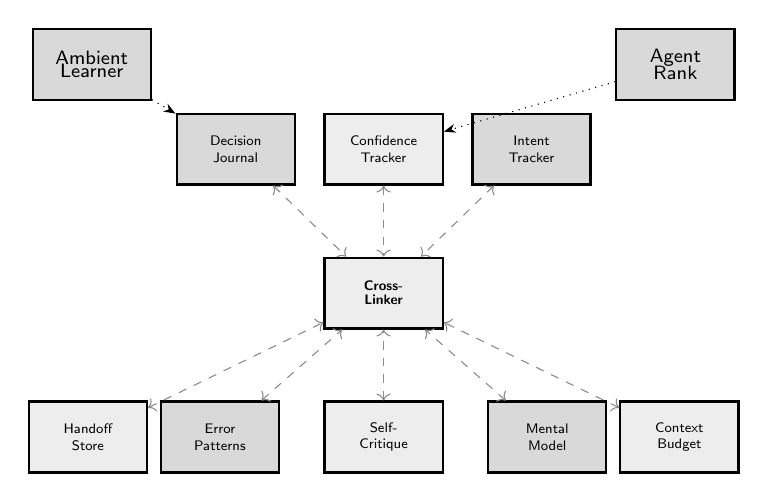
\begin{tikzpicture}[
  node distance=0.45cm and 0.35cm,
  store/.style={draw, thick, minimum width=15mm, minimum height=9mm, font=\sffamily\tiny, align=center, fill=#1},
  link/.style={<->, thin, dashed, color=medgray},
]
  % Top row
  \node[store=lightgray]      (dec)    {Decision\\Journal};
  \node[store=verylightgray, right=of dec]  (conf)   {Confidence\\Tracker};
  \node[store=lightgray, right=of conf] (intent) {Intent\\Tracker};

  % Center
  \node[store=verylightgray, below=0.9cm of conf] (xlink) {\textbf{Cross-}\\[-1pt]\textbf{Linker}};

  % Bottom row
  \node[store=lightgray, below left=0.9cm and 0.55cm of xlink]   (err)   {Error\\Patterns};
  \node[store=verylightgray, below=0.9cm of xlink]               (crit)  {Self-\\Critique};
  \node[store=lightgray, below right=0.9cm and 0.55cm of xlink]  (model) {Mental\\Model};

  % Side stores
  \node[store=verylightgray, left=0.15cm of err] (hand) {Handoff\\Store};
  \node[store=verylightgray, right=0.15cm of model] (budget) {Context\\Budget};

  % Auxiliary
  \node[store=lightgray, above left=0.15cm and 0.3cm of dec] (ambient) {\scriptsize Ambient\\[-1pt]\scriptsize Learner};
  \node[store=lightgray, above right=0.15cm and 0.3cm of intent] (rank) {\scriptsize Agent\\[-1pt]\scriptsize Rank};

  % Links through cross-linker
  \draw[link] (dec) -- (xlink);
  \draw[link] (conf) -- (xlink);
  \draw[link] (intent) -- (xlink);
  \draw[link] (err) -- (xlink);
  \draw[link] (crit) -- (xlink);
  \draw[link] (model) -- (xlink);
  \draw[link] (hand) -- (xlink);
  \draw[link] (budget) -- (xlink);

  \draw[-{Stealth[length=1.5mm]}, thin, dotted] (ambient) -- (dec);
  \draw[-{Stealth[length=1.5mm]}, thin, dotted] (rank) -- (conf);
\end{tikzpicture}}%
\caption{Cognition stores interconnected via CognitionCrossLinker. Dashed arrows: Redis cross-links. Dotted arrows: auxiliary feeds.}
\label{fig:cognition}
\end{figure}

\subsection{Primary Stores}

\subsubsection{DecisionJournal}

Records decisions with structured fields: question, options array with pros/cons, chosen option, reasoning, confidence level, and optional outcome. Supports retrospective evaluation where outcomes are attached after the decision's consequences are observed. Stored at \code{mcp:cognition:decisions:\{id\}}.

\subsubsection{ConfidenceTracker}

Maintains calibrated confidence scores in the range $[0, 1]$ per domain. Each entry includes the score, domain identifier, calibration notes, and trend data (improving, stable, declining). Calibration is computed by comparing predicted confidence to actual outcomes over a sliding window. Stored at \code{mcp:cognition:confidence:\{domain\}}.

\subsubsection{IntentTracker}

Implements hierarchical goal tracking with three levels: mission (top-level objective), goals (concrete milestones), and sub-goals. Drift detection triggers when the current activity diverges from declared goals by more than a configurable threshold. Stored at \code{mcp:cognition:intents:\{id\}}.

\subsubsection{ErrorPatternDB}

A cross-session error database that stores error signatures (type, message pattern, stack fingerprint) with associated context, resolution steps, and recurrence counts. New errors are matched against known patterns using symptom similarity scoring. Stored at \code{mcp:cognition:errors:\{hash\}}.

\subsubsection{SelfCritiqueStore}

Produces structured reflections after task completion. Each critique contains: what went well, what could improve, lessons learned, and action items. Supports check-application queries that retrieve relevant lessons for a given context. Stored at \code{mcp:cognition:critiques:\{id\}}.

\subsubsection{MentalModelStore}

Maintains component-relationship maps representing the agent's understanding of system architecture. Models include: components with descriptions, relationships with types (depends-on, contains, communicates-with), dependency chains, and invariant assertions. Supports impact analysis: given a proposed change, enumerate affected components. Stored at \code{mcp:cognition:models:\{name\}}.

\subsubsection{HandoffStore}

Produces auto-enriched session snapshots for structured context transfer between agents. A handoff report includes: active task summary, key decisions made, files modified, open questions, and recommendations. Enrichment automatically attaches recent cognition state (confidence levels, intent tree, relevant error patterns). Stored at \code{mcp:cognition:handoffs:\{id\}}.

\subsubsection{ContextBudgetManager}

Estimates token consumption for context windows using the approximation of 1~token $\approx$ 4~characters. The manager computes a relevance score for each context item using a weighted average:

\begin{equation}
R = w_r \cdot \text{recency} + w_f \cdot \text{frequency} + w_i \cdot \text{importance}
\label{eq:relevance}
\end{equation}

\noindent with default weights $w_r = 0.4$, $w_f = 0.3$, $w_i = 0.3$. Items below the relevance threshold are suggested for trimming.

\subsection{Auxiliary Components}

\subsubsection{AmbientLearner}

Silently gathers knowledge from tool usage patterns without explicit invocation:

\begin{itemize}[nosep]
\item \emph{Tool sequences}: Records ordered tool invocation chains, identifying common workflows (e.g., \code{git-diff} $\to$ \code{code-review} $\to$ \code{fix-bug}).
\item \emph{File relationships}: Tracks which files are frequently accessed together, building an implicit dependency graph.
\item \emph{Time patterns}: Records temporal patterns (tool usage frequency by time of day, session duration distributions).
\end{itemize}

\subsubsection{AgentRankStore}

Maintains a composite agent ranking system with five tiers: bronze (0--200), silver (201--400), gold (401--600), platinum (601--800), and diamond (801--1000). The composite score is computed as:

\begin{equation}
\text{Score} = 0.4 \cdot S_r + 0.3 \cdot C_t + 0.2 \cdot A_s + 0.1 \cdot C_o
\label{eq:rank}
\end{equation}

\noindent where $S_r$ is the success rate, $C_t$ is task complexity (normalized), $A_s$ is average speed (inverse-normalized), and $C_o$ is collaboration score. Scores decay over time at a rate of $\alpha = 0.95$ per day to reflect recent performance.

\subsection{CognitionCrossLinker}

The CrossLinker maintains bidirectional Redis links between store entries. When a decision is recorded, the CrossLinker creates links to associated confidence scores, intent nodes, and error patterns. Links are stored as Redis sets at \code{mcp:cognition:links:\{source\}} and \code{mcp:cognition:links:\{target\}}, enabling both forward and reverse traversal.

\subsection{Reactive Event Handlers}

Nine reactive handlers on the GlobalEventBus create a feedback loop between cognition stores:

\begin{enumerate}[nosep]
\item \code{decision:recorded} $\to$ Auto-create confidence record and cross-link.
\item \code{confidence:low} $\to$ Check intent drift.
\item \code{error:recorded} $\to$ Scan recent decisions for causal links.
\item \code{error:matched} $\to$ Log known fix suggestion.
\item \code{critique:lesson-learned} $\to$ Link to matching error patterns.
\item \code{intent:drifted} $\to$ Trigger self-critique.
\item \code{handoff:created} $\to$ Link relevant mental models.
\item \code{model:stale} $\to$ Flag affected decisions and intents.
\item \code{confidence:outcome} $\to$ Propagate to linked decisions.
\end{enumerate}

% ══════════════════════════════════════════════════════════════════
\section{Tool Categories}
\label{sec:tools}

Table~\ref{tab:tools} enumerates all 23~tool categories with counts and representative tools.

\begin{table}[!t]
\centering
\caption{Tool Categories (142 Total)}
\label{tab:tools}
\renewcommand{\arraystretch}{0.95}
\begin{tabular}{@{}lcp{28mm}@{}}
\toprule
\textbf{Category} & \textbf{\#} & \textbf{Key Tools} \\
\midrule
Cluster Bus       & 7  & \code{bus-status}, \code{-magistrale} \\
Cognition         & 8  & \code{decision-journal}, \code{confidence} \\
AI Agents         & 4  & \code{plan}, \code{build}, \code{brainstorm} \\
Multi-LLM         & 3  & \code{multi-prompt}, \code{consensus} \\
Code Analysis     & 8  & \code{code-review}, \code{find-def} \\
Line Editing      & 4  & \code{insert-at-line}, \code{replace-lines} \\
Symbol Editing    & 3  & \code{rename-symbol}, \code{insert-after} \\
Code Mod.         & 5  & \code{fix-bug}, \code{refactor}, \code{auto-fix} \\
Project Memory    & 8  & \code{write-memory}, \code{checkpoint-save} \\
Git               & 8  & \code{git-status}, \code{git-diff}, \code{git-log} \\
File Operations   & 9  & \code{file-read}, \code{file-write}, \code{file-search} \\
Project           & 5  & \code{run-tests}, \code{run-lint}, \code{check-types} \\
Kanban Tasks      & 12 & \code{task-create}, \code{task-claim} \\
Kanban Workspaces & 5  & \code{workspace-create}, \code{-join} \\
Kanban Boards     & 6  & \code{board-create}, \code{board-share} \\
Recursive         & 4  & \code{invoke-tool}, \code{orchestrate} \\
Multi-Agent       & 14 & \code{agent-register}, \code{shared-thoughts} \\
Pipeline          & 1  & \code{pipeline} \\
Session           & 6  & \code{session-recover}, \code{session-create} \\
MCP Client        & 3  & \code{client-sampling}, \code{client-elicit} \\
Knowledge Graph   & 4  & \code{graph-query}, \code{loci-recall} \\
Thinking          & 1  & \code{thinking-chain} \\
MPC Security      & 4  & \code{mpc-split}, \code{mpc-reconstruct} \\
RL Learning       & 2  & \code{rl-reward-stats} \\
System            & 8  & \code{env-info}, \code{tool-health}, \code{ping} \\
\bottomrule
\end{tabular}
\end{table}

% ══════════════════════════════════════════════════════════════════
\section{Multi-Agent Coordination}
\label{sec:multiagent}

KemdiCode supports multi-agent workflows where multiple AI sessions collaborate on shared tasks through four mechanisms:

\begin{description}[nosep,style=unboxed,leftmargin=0pt,font=\normalfont\itshape]
\item[Agent Registry.] Agents register with role (supervisor, worker, observer), capabilities, and status. Discovery is via \code{agent-list}; real-time monitoring via \code{agent-watch}.

\item[Message Passing.] \code{agent-inject} sends context to specific agents via Redis Pub/Sub (\code{inject:\{agentId\}}). \code{agent-alert} broadcasts to all agents on the \code{alerts} channel. \code{shared-thoughts} provides a collective knowledge base accessible by all agents.

\item[Kanban System.] Hierarchical task management: workspaces contain boards, boards contain tasks. Tasks support claiming, assignment, comments, and status transitions (\code{pending} $\to$ \code{in\_progress} $\to$ \code{completed}). Role-based membership (owner, admin, member, viewer) controls access at the board level.

\item[Task Intelligence.] \code{task-cluster} uses LLM-driven semantic clustering to group related tasks. \code{task-complexity} provides AI-powered difficulty estimation with priority scoring.
\end{description}

% ══════════════════════════════════════════════════════════════════
\section{Security}
\label{sec:security}

\subsection{Input Validation}

All tool inputs are validated via Zod schemas before execution. File paths undergo traversal protection through \code{validatePathSafe()}, which rejects paths containing \code{..} traversal sequences, null bytes, and paths outside the session's working directory.

\subsection{Redis Security}

JSON parsing from Redis employs prototype pollution protection, blocking dangerous keys: \code{\_\_proto\_\_}, \code{constructor}, and \code{prototype}. This prevents injection of properties into JavaScript's object prototype chain.

\subsection{Cluster Bus Authentication}

As described in Section~\ref{sec:l3}, all cluster signals are HMAC-SHA256 authenticated with constant-time comparison. The shared key is configured at server start and is never transmitted over the bus.

\subsection{Multi-Party Computation}

Shamir's Secret Sharing~\cite{shamir1979} enables distributed secret management:

\begin{enumerate}[nosep]
\item \code{mpc-split}: Split secret into $n$ shares with threshold $t$.
\item \code{mpc-distribute}: Distribute shares to agents via encrypted channels.
\item \code{mpc-reconstruct}: Reconstruct from $\geq t$ shares.
\end{enumerate}

\subsection{Anti-ReDoS}

MetaRouter regex patterns are capped at 200~characters, preventing Regular Expression Denial of Service attacks through pathological backtracking.

% ══════════════════════════════════════════════════════════════════
\section{LLM Provider Integration}
\label{sec:providers}

KemdiCode integrates eight LLM providers through a unified routing layer with the model specification syntax \code{provider:model:thinking}. Table~\ref{tab:providers} summarizes the supported providers.

\begin{table}[!t]
\centering
\caption{LLM Providers}
\label{tab:providers}
\begin{tabular}{@{}llcl@{}}
\toprule
\textbf{Provider} & \textbf{Alias} & \textbf{SDK} & \textbf{Notes} \\
\midrule
Anthropic   & \code{a} & Native  & Extended thinking \\
OpenAI      & \code{o} & Native  & Structured output \\
Gemini      & \code{g} & Native  & Flash/Pro/Ultra \\
Groq        & \code{q} & Compat. & Fast inference \\
DeepSeek    & \code{d} & Compat. & V3, R1 \\
Ollama      & \code{l} & Compat. & Local models \\
OpenRouter  & \code{r} & Compat. & 100+ models \\
Perplexity  & \code{p} & Compat. & Search-augmented \\
\bottomrule
\end{tabular}
\end{table}

The routing layer provides three-tier model selection: primary model for standard requests, research model for complex analysis, and fallback model for quota exhaustion or provider errors. Provider connections are lazily initialized and support hot-reload without server restart.

Structured output is produced via \code{generateObject()}, which combines Zod schemas with \code{jsonrepair} to handle malformed LLM JSON output. This provides reliable typed data extraction across all providers regardless of their native structured output support.

% ══════════════════════════════════════════════════════════════════
\section{Evaluation}
\label{sec:eval}

\subsection{Test Suite}

The system is validated by a comprehensive test suite of 559~passing tests covering all tool categories, bus layers, cognition stores, and edge cases. Tests are executed via \code{bun test} with the Bun runtime.

\subsection{Client Compatibility}

KemdiCode MCP Server has been verified with four MCP clients: Claude Code (primary), Cursor, KiroCode, and RooCode. All clients successfully discover tools, invoke them, and receive SSE notifications without modification.

\subsection{Infrastructure}

The server supports two runtimes (Bun and Node.js) through a runtime abstraction layer that provides unified interfaces for HTTP serving, process management, and cryptographic operations. Tree-sitter~\cite{treesitter} WASM parsers provide AST-based code analysis for 19~programming languages.

All persistent state uses Redis DB~2 with 10~key namespaces (\code{mcp:context:*}, \code{mcp:agents:*}, \code{mcp:messages:*}, \code{mcp:kanban:*}, \code{mcp:memory:*}, \code{mcp:cognition:*}, \code{mcp:cluster:*}, \code{mcp:dataflow:*}, \code{mcp:events:*}, \code{mcp:channel:*}).

\subsection{Performance Characteristics}

\begin{itemize}[nosep]
\item Lazy schema loading eliminates startup latency for unused tools.
\item O(1) subscribe/unsubscribe operations on both DataFlowBus and HealthMonitor via \code{Map}-based tracking.
\item Circuit breakers in the SignalFlowController prevent cascade failures.
\item Bloom filter deduplication uses 35\,KB for 20{,}000-item capacity at 0.1\% false-positive rate.
\item Idle subscription cleanup after 60~minutes prevents resource leaks.
\end{itemize}

% ══════════════════════════════════════════════════════════════════
\section{Conclusion}
\label{sec:conclusion}

KemdiCode MCP Server v1.25.0 demonstrates that the Model Context Protocol can serve as a foundation for comprehensive AI-assisted software engineering platforms. By combining 142~specialized tools, a three-layer distributed bus architecture with formalized anti-amplification guards, a persistent cognition system with reactive cross-linking, and multi-provider LLM orchestration with quality-driven aggregation, the server transforms MCP from a simple tool-calling interface into a stateful, distributed AI development infrastructure.

The three-layer bus design (\layerthree~ClusterBus, \layertwo~DataFlowBus, \layerone~GlobalEventBus) provides clear separation of concerns: inter-cluster communication with cryptographic authentication, typed inter-module messaging with schema validation, and efficient in-process event propagation with cascade protection. The anti-amplification bridge mechanism, formalized through hop counters, source guards, deduplication sets, and chain-depth limits, ensures system stability under complex multi-layer message flows.

The architecture draws on established distributed systems techniques~\cite{lamport1978,bloom1970} and recent advances in LLM-based multi-agent coordination~\cite{li2024multiagent,guo2024ijcai}. Future work includes expanding the knowledge graph with cross-project learning, adding WebSocket transport support, and deepening the reinforcement learning subsystem for autonomous tool selection optimization.

% ══════════════════════════════════════════════════════════════════
\begin{thebibliography}{15}

\bibitem{mcp2024}
Anthropic, ``Introducing the Model Context Protocol,'' Anthropic Blog, Nov.\ 2024. [Online]. Available: \url{https://www.anthropic.com/news/model-context-protocol}

\bibitem{mcpspec2025}
Model Context Protocol Authors, ``Model Context Protocol Specification, version 2025-11-25,'' 2025. [Online]. Available: \url{https://modelcontextprotocol.io/specification/2025-11-25}

\bibitem{jsonrpc2}
JSON-RPC Working Group, ``JSON-RPC 2.0 Specification,'' 2010. [Online]. Available: \url{https://www.jsonrpc.org/specification}

\bibitem{lsp2016}
Microsoft, Red Hat, and Codenvy, ``Language Server Protocol Specification,'' 2016. [Online]. Available: \url{https://microsoft.github.io/language-server-protocol/}

\bibitem{redis}
S.~Sanfilippo, ``Redis: An in-memory data structure store,'' 2009--2026. [Online]. Available: \url{https://redis.io/}

\bibitem{shamir1979}
A.~Shamir, ``How to share a secret,'' \emph{Commun. ACM}, vol.~22, no.~11, pp.~612--613, Nov.\ 1979. \doi{10.1145/359168.359176}

\bibitem{wagner1998}
T.~A.~Wagner and S.~L.~Graham, ``Efficient and flexible incremental parsing,'' \emph{ACM Trans.\ Program.\ Lang.\ Syst.}, vol.~20, no.~5, pp.~980--1013, Sep.\ 1998. \doi{10.1145/293677.293678}

\bibitem{treesitter}
M.~Brunsfeld \emph{et al.}, ``Tree-sitter: An incremental parsing system for programming tools,'' 2018--2026. [Online]. Available: \url{https://tree-sitter.github.io/}

\bibitem{zod}
C.~Hacks, ``Zod: TypeScript-first schema validation with static type inference,'' 2020--2026. [Online]. Available: \url{https://zod.dev/}

\bibitem{li2024multiagent}
J.~Li, Q.~Wang \emph{et al.}, ``A survey on LLM-based multi-agent systems: Workflow, infrastructure, and challenges,'' \emph{Vicinagearth}, Oct.\ 2024. \doi{10.1007/s44336-024-00009-2}

\bibitem{guo2024ijcai}
T.~Guo, X.~Chen \emph{et al.}, ``Large language model based multi-agents: A survey of progress and challenges,'' in \emph{Proc.\ 33rd Int.\ Joint Conf.\ Artif.\ Intell.\ (IJCAI)}, 2024.

\bibitem{wu2023autogen}
Q.~Wu, G.~Banber \emph{et al.}, ``AutoGen: Enabling next-gen LLM applications via multi-agent conversation,'' \emph{arXiv:2308.08155}, 2023.

\bibitem{hong2023metagpt}
S.~Hong, X.~Zhuge \emph{et al.}, ``MetaGPT: Meta programming for multi-agent collaborative framework,'' \emph{arXiv:2308.00352}, 2023.

\bibitem{bloom1970}
B.~H.~Bloom, ``Space/time trade-offs in hash coding with allowable errors,'' \emph{Commun. ACM}, vol.~13, no.~7, pp.~422--426, Jul.\ 1970. \doi{10.1145/362686.362692}

\bibitem{lamport1978}
L.~Lamport, ``Time, clocks, and the ordering of events in a distributed system,'' \emph{Commun. ACM}, vol.~21, no.~7, pp.~558--565, Jul.\ 1978. \doi{10.1145/359545.359563}

\end{thebibliography}

\end{document}
